\chapter{Implementació i Resultats}

\section{Mètriques analitzades}

\subsection{Mètriques provinents de les Màquines-Servidors}

Abans de procedir a executar el test de càrrega amb diferents arguments, és necessari decidir què analitzarem amb \textit{Netdata} per tal d'esbrinar quin és el coll d'ampolla dels nostres servidors en les dues màquines. Aquesta aplicació web ofereix gràfics de centenars de mètriques, però els components a analitzar estan clars. Ens interessa una mètrica que ens indiqui l'estat del processador, l'estat de la memòria lliure i l'estat de l'entrada i sortida d'informació per internet. Afortunadament, existeixen tres mètriques que ens proporcionen la informació adequada per a cada aspecte: la primera és \textit{system.cpu}, que mostra un gràfic del percentatge d'ús del processador. La segona és \textit{mem.available}, que mostra la memòria lliure en \textit{mebibytes} disponible per ser utilitzada pels processos del sistema operatiu. La tercera és \textit{system.net}, que mostra la quantitat de kilobits per segon enviats en vermell i la quantitat de kilobits per segon rebuts en verd.

A més, Netdata proporciona unes mètriques anomenades \textit{Pressure Stall Information}\cite{noauthor_pressure_2024}, que recopilen informació proporcionada per \textit{Linux} sobre la quantitat de temps que alguna tasca ha estat parada a causa de la falta d'algun recurs\cite{weiner_psi_2018}. En particular, les gràfiques són: \textit{system.io\_some\_pressure\_stall\_time}, que mostra els mil·lisegons que algun procés ha estat aturat perquè el recurs requerit per a l'entrada/sortida ja estava ocupat; \textit{system.cpu\_some\_pressure\_stall\_time}, que mostra els mil·lisegons que algun procés ha estat aturat perquè el processador estava ocupat; i finalment, \textit{system.memory\_some\_pressure\_stall\_time}, que mostra la quantitat de mil·lisegons que algun procés ha estat aturat perquè la \textit{RAM} estava ocupada.

\subsection{Mètriques provinents de la Màquina-Client}

\textit{k6} proporciona un resum cada cop que finalitza una execució, anomenat \textit{end-of-test summary}, que ofereix molta informació sobre el rendiment percebut per cada \textit{VU}, la quantitat total de MB enviats i rebuts, els percentils i les mitjanes del temps de resposta de diferents peticions HTTP, la duració total d'una iteració, etc.\cite{grafana_results_nodate}. Els factors als quals s'ha considerat donar especial atenció per a aquesta anàlisi són els següents:
\begin{itemize}
    \item checks: descriu el percentatge de peticions que han complert tots els checks definits per les \textit{VUs}.
    \item http\_req\_duration: indica la distribució temporal de totes les peticions \textit{HTTP} realitzades.
    \item http\_req\_failed: descriu el percentatge de peticions \textit{HTTP} que han fallat o que no han complert amb el \textit{threshold} establert.
    \item iteration\_duration: mostra la distribució temporal d'una iteració d'una \textit{VU}.
\end{itemize}
Amb aquestes dades, podrem avaluar objectivament si una màquina ha tingut un millor rendiment que una altra, basant-nos en el percentatge de peticions servides correctament, el temps de resposta de les peticions, la duració total d'una iteració i el percentatge de peticions fallides o que no han complert el \textit{threshold} establert

\newpage
\section{Resultats}
\label{11:resultats}

\subsection{Test 1}

El primer test és amb molt poca càrrega, que simula fins a 20 usuaris generant una càrrega de treball cada 5 segons.

\subsubsection{Màquina al núvol}
Consisteix en la següent comanda al \textit{Powershell}:
\begin{lstlisting}[language=bash, caption=Test 1 al núvol]
    $env:K6_CLOUD=1; $env:K6_PRIMER=10;$env:K6_MIG=20; k6 run .\script.js
\end{lstlisting}

\begin{figure}[!htbp]
    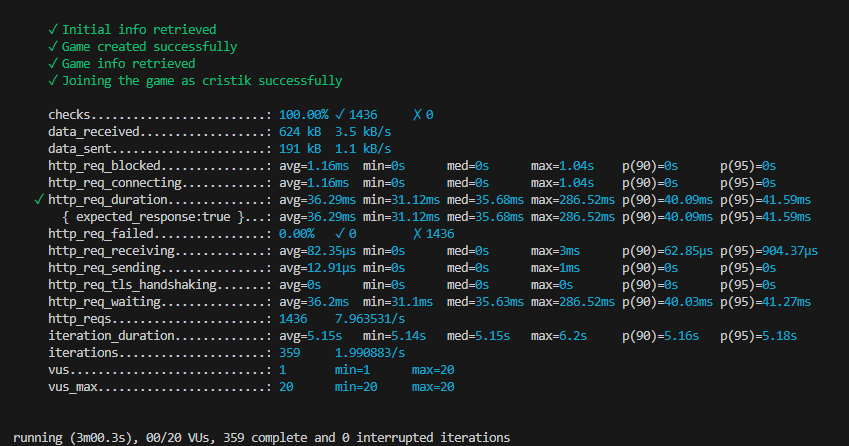
\includegraphics[width=1\textwidth]{Imatges/Tests/Núvol/1c-k6.png}  
    \caption{\textit{end-of-test summary} del Test 1 al núvol}
\end{figure}

\begin{figure}[!htbp]
    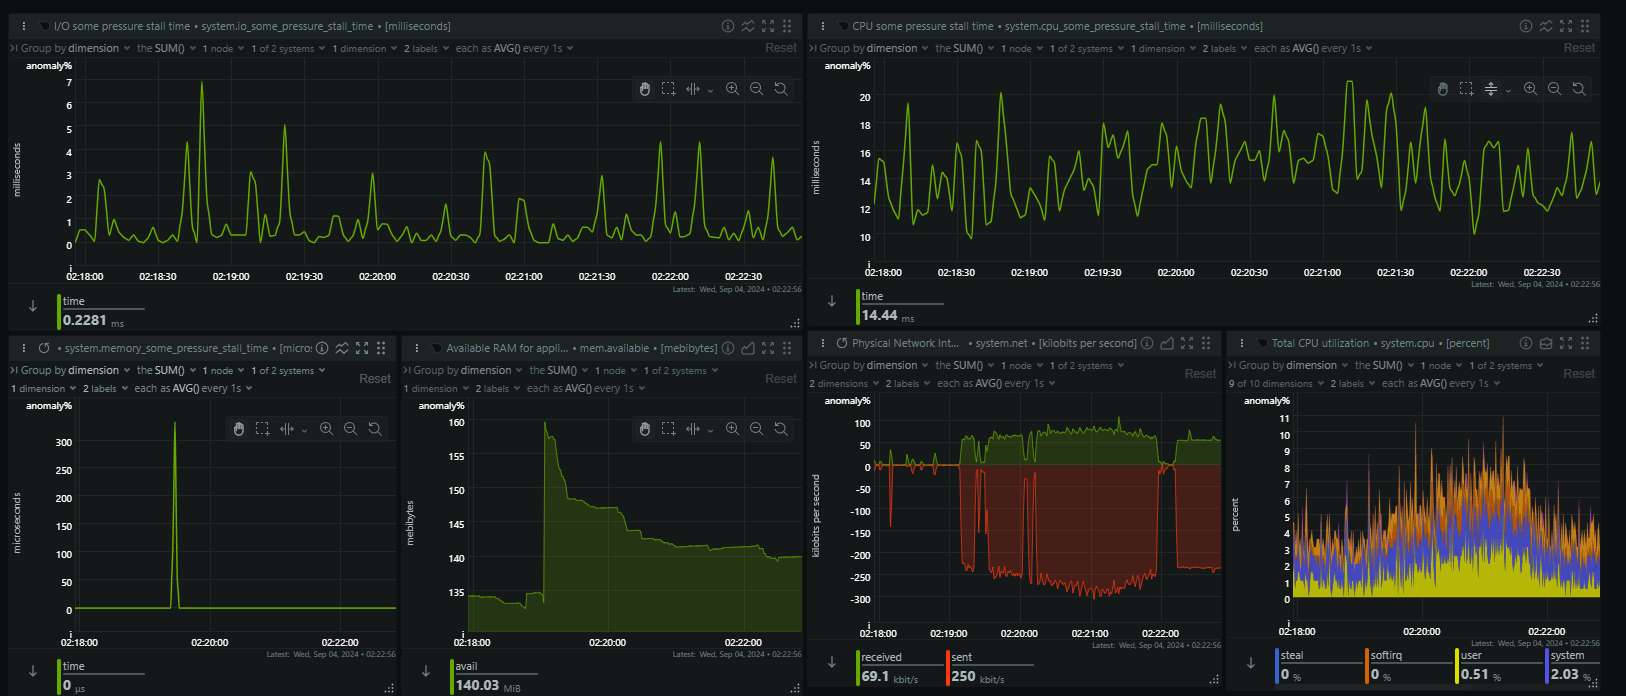
\includegraphics[width=1\textwidth]{Imatges/Tests/Núvol/1c-netdata.png}  
    \caption{Tauler de \textit{Netdata} del Test 1 al núvol}
\end{figure}

\subsubsection{Màquina local}
Consisteix en la següent comanda al \textit{Powershell}:
\begin{lstlisting}[language=bash, caption=Test 1 local]
    $env:K6_CLOUD=0; $env:K6_PRIMER=10;$env:K6_MIG=20; k6 run .\script.js
\end{lstlisting}

\begin{figure}[!htbp]
    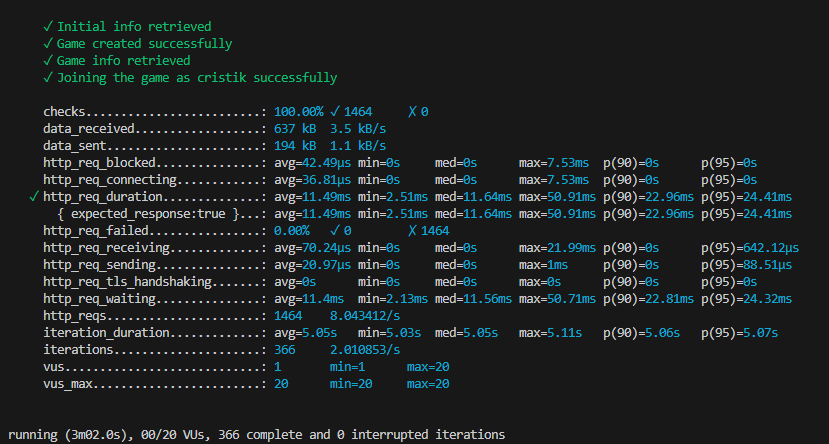
\includegraphics[width=1\textwidth]{Imatges/Tests/Local/1l-k6.png}  
    \caption{\textit{end-of-test summary} del Test 1 local}
\end{figure}

\begin{figure}[!htbp]
    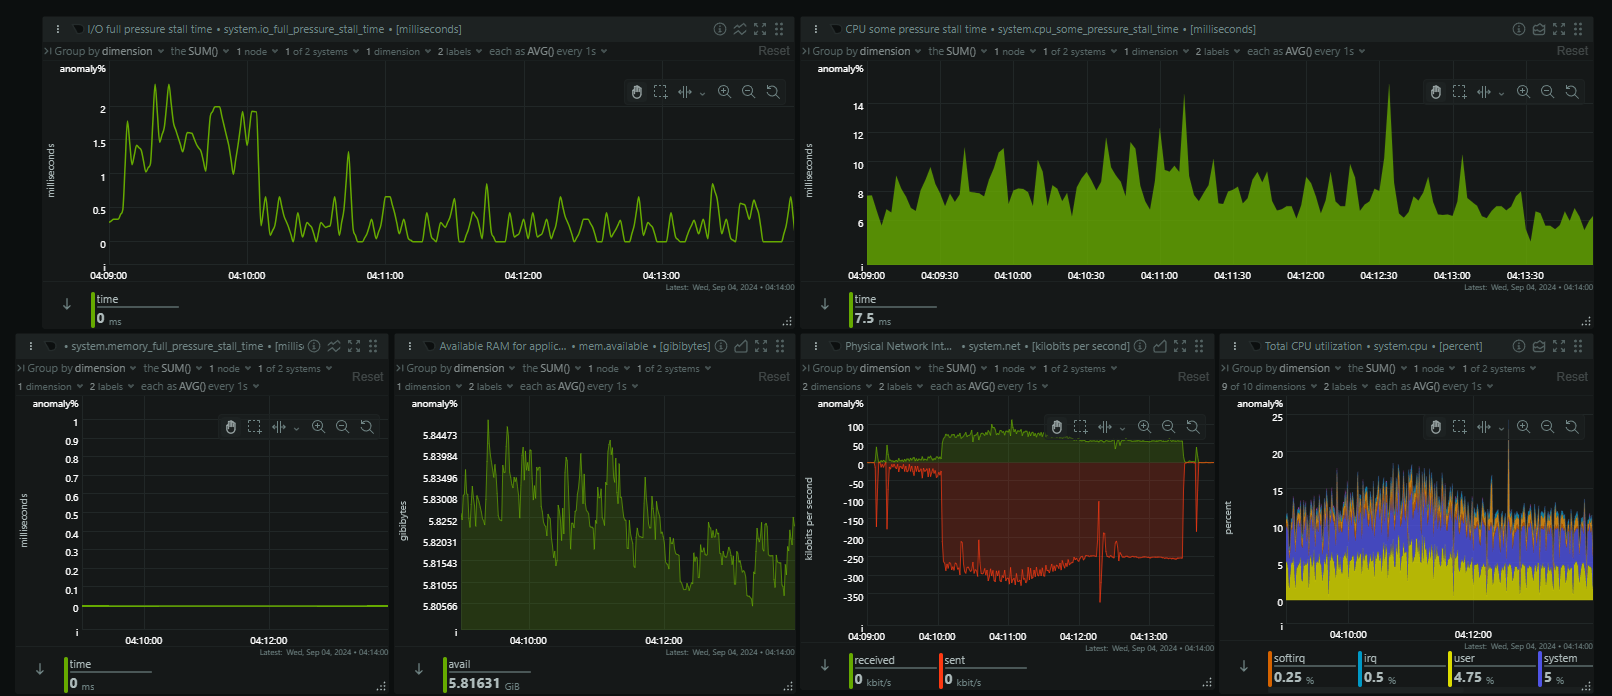
\includegraphics[width=1\textwidth]{Imatges/Tests/Local/1l-netdata.png}  
    \caption{Tauler de \textit{Netdata} del Test 1 local}
\end{figure}

\subsubsection{Conclusió del test}

En aquesta primera prova, es pot veure que ambdues màquines responen correctament a aproximadament 360 iteracions i 1.450 peticions en un període de 3 minuts. La màquina local és aproximadament dues o tres vegades més ràpida a l'hora de retornar la resposta en comparació amb la màquina al núvol. Tot i això, cap de les dues màquines ha tingut \textit{VUs} que hagin superat els 0,5 segons de mitjana en el conjunt de les seves iteracions, ja que aquestes es comptarien com a fallades en la mètrica \textit{http\_req\_failed}.

Als taulers de \textit{Netdata} no s'observa cap carència significativa en cap de les dues màquines. Tots els recursos estan per sota del seu límit, i el retard a causa de la pressió no varia gaire respecte al comportament habitual.

\newpage
\subsection{Test 2}

El segon test té una càrrega moderada, que simula fins a 200 usuaris generant una càrrega de treball cada 5 segons.

\subsubsection{Màquina al núvol}
Consisteix en la següent comanda al \textit{Powershell}:
\begin{lstlisting}[language=bash, caption=Test 2 al núvol]
    $env:K6_CLOUD=1; $env:K6_PRIMER=100;$env:K6_MIG=200; k6 run .\script.js
\end{lstlisting}

\begin{figure}[!htbp]
    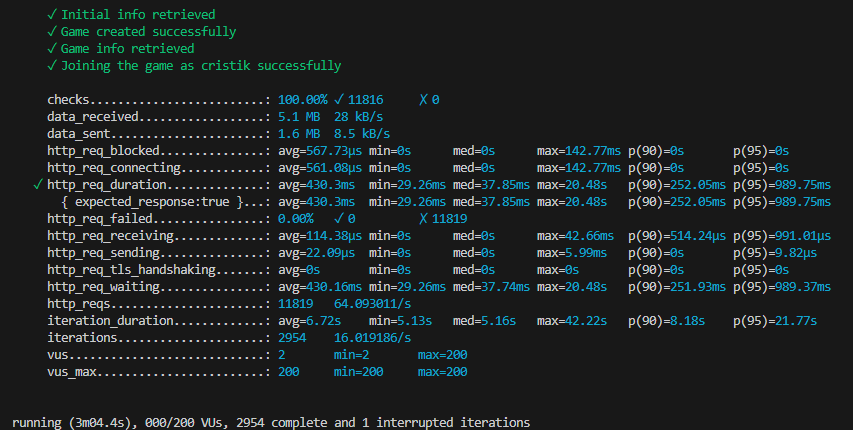
\includegraphics[width=1\textwidth]{Imatges/Tests/Núvol/2c-k6.png}  
    \caption{\textit{end-of-test summary} del Test 2 al núvol}
\end{figure}

\begin{figure}[!htbp]
    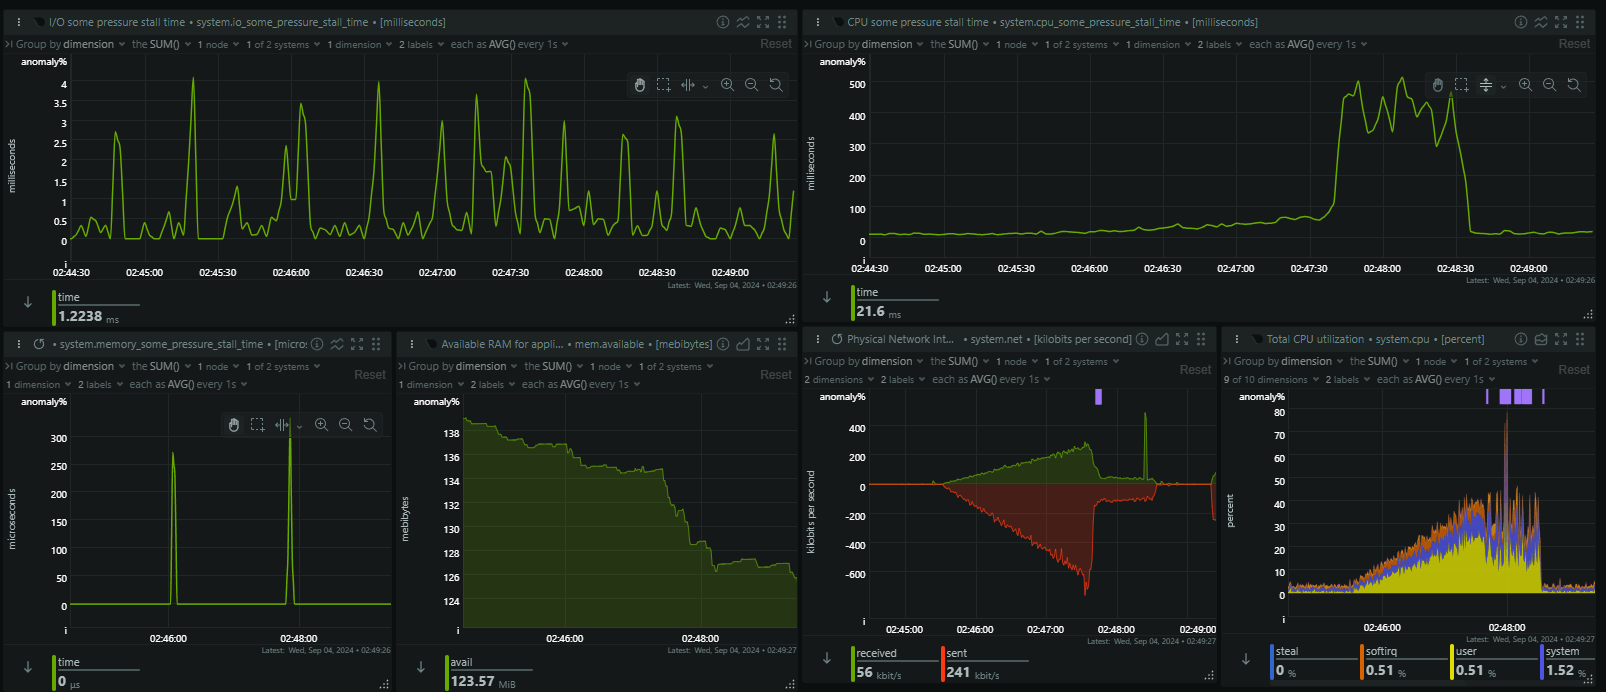
\includegraphics[width=1\textwidth]{Imatges/Tests/Núvol/2c-netdata.png}  
    \caption{Tauler de \textit{Netdata} del Test 2 al núvol}
\end{figure}

\subsubsection{Màquina local}
Consisteix en la següent comanda al \textit{Powershell}:
\begin{lstlisting}[language=bash, caption=Test 2 local]
    $env:K6_CLOUD=0; $env:K6_PRIMER=100;$env:K6_MIG=200; k6 run .\script.js
\end{lstlisting}

\begin{figure}[!htbp]
    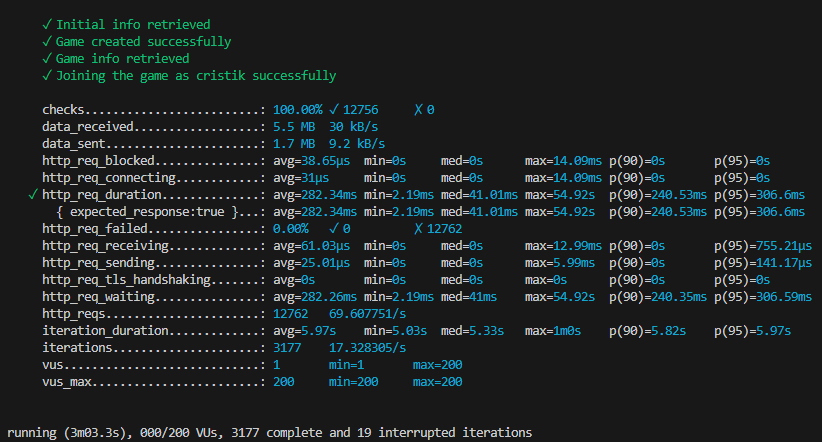
\includegraphics[width=1\textwidth]{Imatges/Tests/Local/2l-k6.png}  
    \caption{\textit{end-of-test summary} del Test 2 local}
\end{figure}

\begin{figure}[!htbp]
    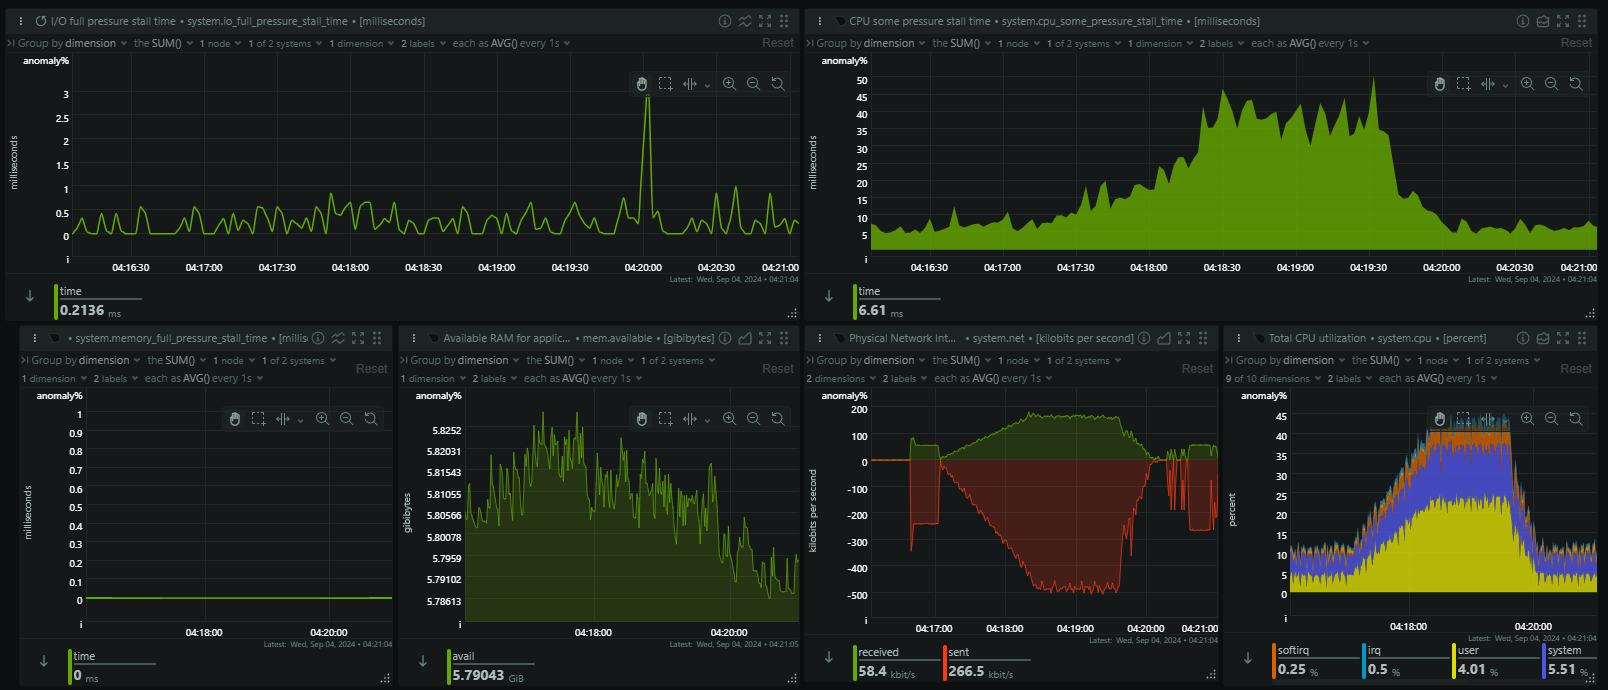
\includegraphics[width=1\textwidth]{Imatges/Tests/Local/2l-netdata.png}  
    \caption{Tauler de \textit{Netdata} del Test 2 local}
\end{figure}

\subsubsection{Conclusió del test}

En aquesta segona prova, igual que en la primera, ambdues màquines són capaces de gestionar el trànsit de manera efectiva, sense cap error i dins del termini establert de 500 ms com a mitjana per a cada \textit{VU}. El temps de latència continua afavorint clarament la màquina local, que respon a les peticions aproximadament dues o tres vegades més ràpidament que la màquina al núvol. A més, la duració total d'una iteració també beneficia la màquina local, excloent els 5 segons de pausa en què la iteració es manté inactiva.

Al tauler de \textit{Netdata}, es pot observar una diferència significativa en el retard causat per la pressió sobre el processador. Mentre que la màquina local experimenta un retard d'aproximadament 50 ms, la màquina al núvol pateix un col·lapse a les 2:47:30, on el retard s'incrementa bruscament fins als 500 ms. Al mateix temps, la quantitat de paquets enviats i rebuts cau dràsticament, fins a només 20 kbps d'entrada i 100 kbps de sortida. Aquest col·lapse coincideix amb el moment més intensiu del test, on es simulen 200 \textit{VUs}.

\newpage
\subsection{Test 3}

El tercer test té una càrrega alta, que simula fins a 2000 usuaris generant una càrrega de treball cada 5 segons.

\subsubsection{Màquina al núvol}
Consisteix en la següent comanda al \textit{Powershell}:
\begin{lstlisting}[language=bash, caption=Test 3 al núvol]
    $env:K6_CLOUD=1; $env:K6_PRIMER=1000;$env:K6_MIG=2000; k6 run .\script.js
\end{lstlisting}

\begin{figure}[!htbp]
    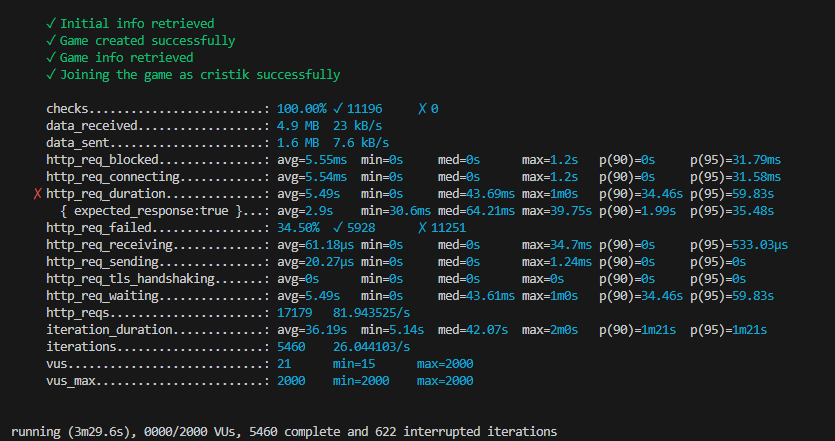
\includegraphics[width=1\textwidth]{Imatges/Tests/Núvol/3c-k6.png}  
    \caption{\textit{end-of-test summary} del Test 3 al núvol}
\end{figure}

\begin{figure}[!htbp]
    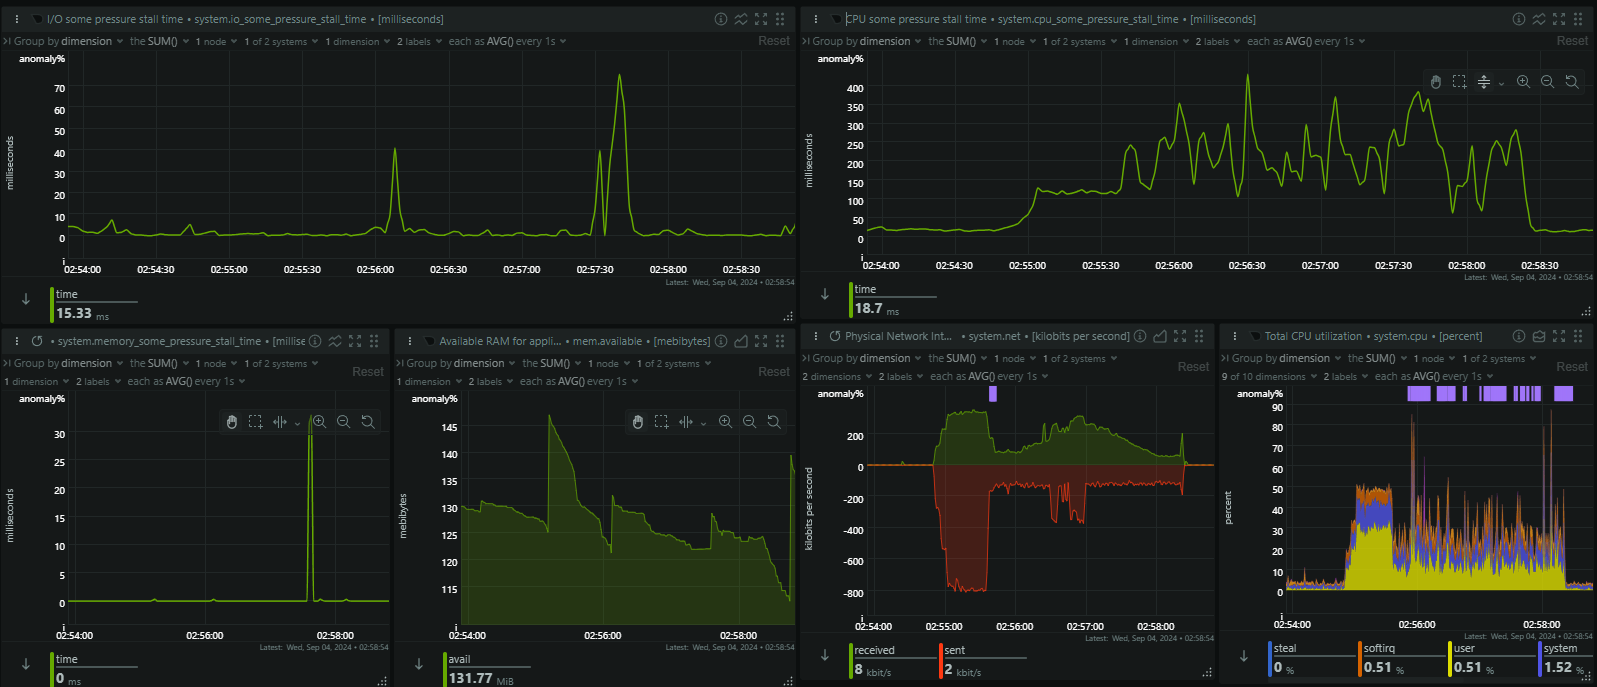
\includegraphics[width=1\textwidth]{Imatges/Tests/Núvol/3c-netdata.png}  
    \caption{Tauler de \textit{Netdata} del Test 3 al núvol}
\end{figure}

\subsubsection{Màquina local}
Consisteix en la següent comanda al \textit{Powershell}:
\begin{lstlisting}[language=bash, caption=Test 3 local]
    $env:K6_CLOUD=0; $env:K6_PRIMER=1000;$env:K6_MIG=2000; k6 run .\script.js
\end{lstlisting}

\begin{figure}[!htbp]
    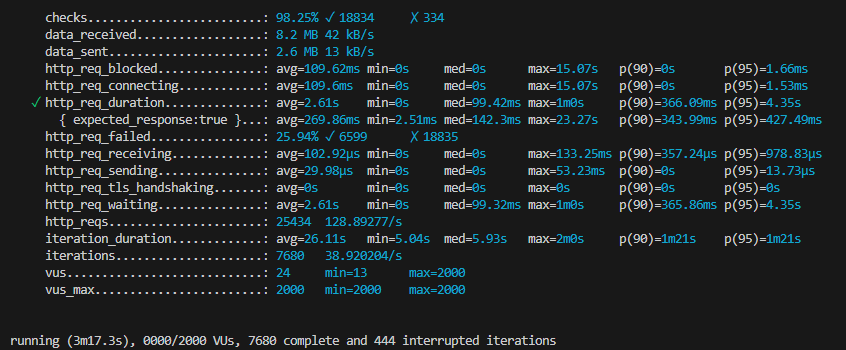
\includegraphics[width=1\textwidth]{Imatges/Tests/Local/3l-k6.png}  
    \caption{\textit{end-of-test summary} del Test 3 local}
\end{figure}

\begin{figure}[!htbp]
    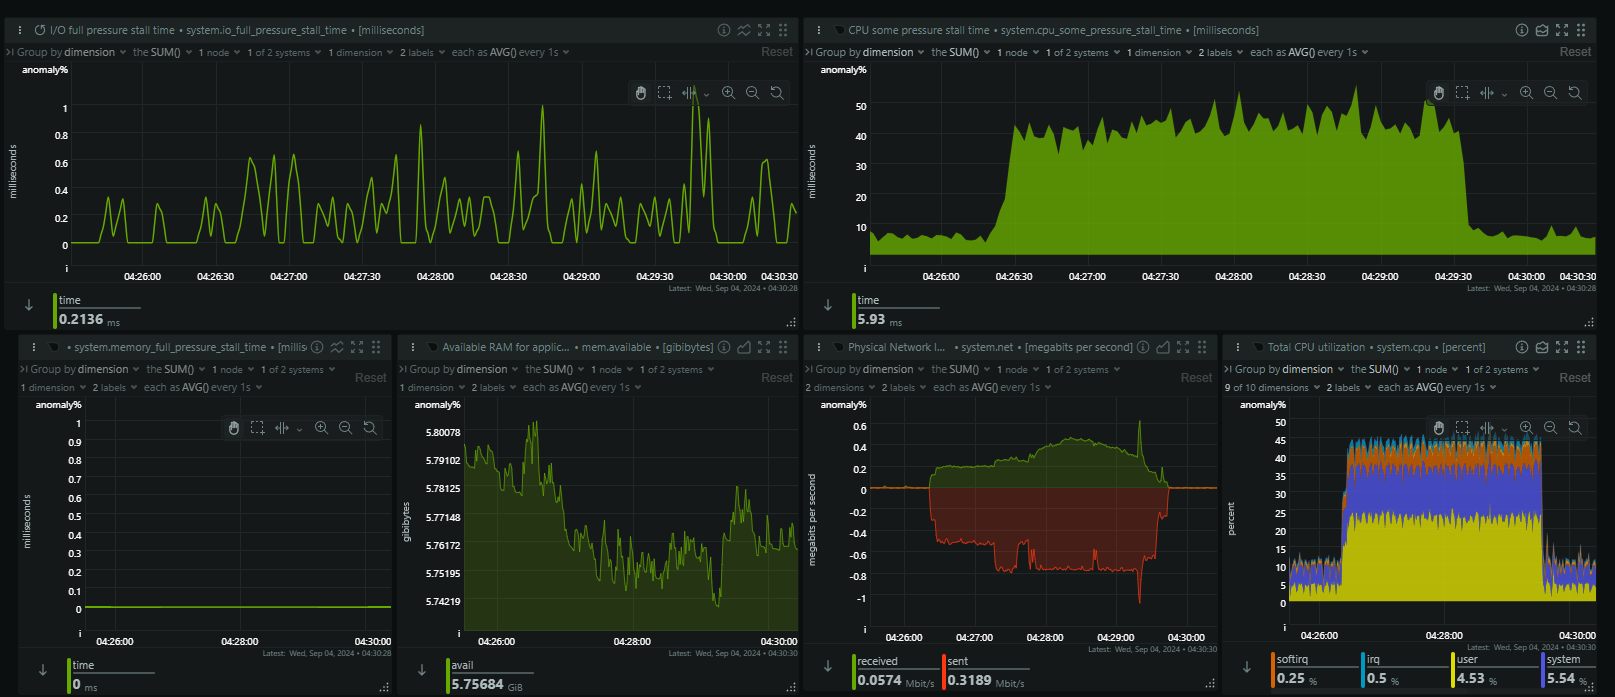
\includegraphics[width=1\textwidth]{Imatges/Tests/Local/3l-netdata.png}  
    \caption{Tauler de \textit{Netdata} del Test 3 local}
\end{figure}
\subsubsection{Conclusió del test}

En aquesta tercera prova, per primera vegada, es poden observar tests que fallen tant en els \textit{checks} com en les peticions \textit{HTTP} a la màquina local, així com fallades \textit{HTTP} a la màquina del núvol. En aquesta prova, la diferència en el nombre d'iteracions completades entre la màquina local (7.600) i la màquina del núvol (5.460) s'ha ampliat significativament. Una sorpresa d'aquesta prova és que la màquina al núvol ha enviat codis de resposta \textit{200 OK} a totes les seves respostes, i, per tant, tots els \textit{checks} han estat correctes. Una possible hipòtesi per explicar aquest fenomen podria ser que el núvol controli les peticions de tornada de la màquina i descarti les que retornin un error. Això podria explicar la gran diferència en el nombre d'iteracions en aquesta prova i el fet que tots els \textit{checks} siguin correctes (ja que, si la resposta no arriba mai, no s'executa el \textit{check}).

D'altra banda, la màquina local sí que ha respost amb errors en algunes de les peticions del client, cosa que indica que la màquina local ja no té la capacitat per gestionar tot el trànsit. A més del nombre d'iteracions completades, el nombre d'iteracions interrompudes reflecteix el nombre de \textit{VUs} que no han pogut acabar la seva iteració iniciada durant els 3 minuts de prova, més el temps addicional donat dinàmicament a els \textit{VUs} per acabar de manera natural la seva iteració, abans que es forcin a aturar. Aquest número és una bona indicació per estimar quantes \textit{VUs} s'han quedat sense resposta, ja sigui perquè el temps addicional no ha estat suficient per completar la iteració, o perquè alguna resposta s'ha perdut. El fet que la màquina al núvol tingui aproximadament 200 \textit{VUs} forçosament interrompudes podria ser una evidència a favor de la hipòtesi anterior, en què els \textit{VUs} no aconsegueixen completar les seves iteracions perquè no arriben a rebre les respostes amb errors.

Al tauler de \textit{Netdata}, es pot observar que la màquina al núvol continua sent limitada pel processador, generant un retràs d'uns 200 ms durant tota l'execució de la prova. També es poden veure alguns pics de retràs de 50 ms en els components d'entrada/sortida. En general, es nota que la connexió a Internet de la màquina al núvol també colapsa. Al començament de la prova, es reben fins a 300 kbps i s'envien fins a 800 kbps, però a partir del primer minut, quan el nombre de \textit{VUs} augmenta de 1.000 a 2.000, aquestes velocitats disminueixen en lloc d'augmentar, coincidint amb els pics més alts de retràs del processador.

D'altra banda, la màquina local té un retràs mitjà de 40 ms a causa del processador, però la connexió millora a mesura que avança el test, amb 400 kbps de dades rebudes i 800 kbps enviades. Amb aquesta informació, podem hipotetitzar que el col·lapse de la connexió a la màquina al núvol es deu majoritàriament al gran retràs en el processament dels missatges.

\newpage
\subsection{Test 4}

El quart test té una càrrega molt alta, que simula fins a 10000 usuaris generant una càrrega de treball cada 5 segons.

\subsubsection{Màquina al núvol}
Consisteix en la següent comanda al \textit{Powershell}:
\begin{lstlisting}[language=bash, caption=Test 4 al núvol]
    $env:K6_CLOUD=1; $env:K6_PRIMER=5000;$env:K6_MIG=10000; k6 run .\script.js
\end{lstlisting}

\begin{figure}[!htbp]
    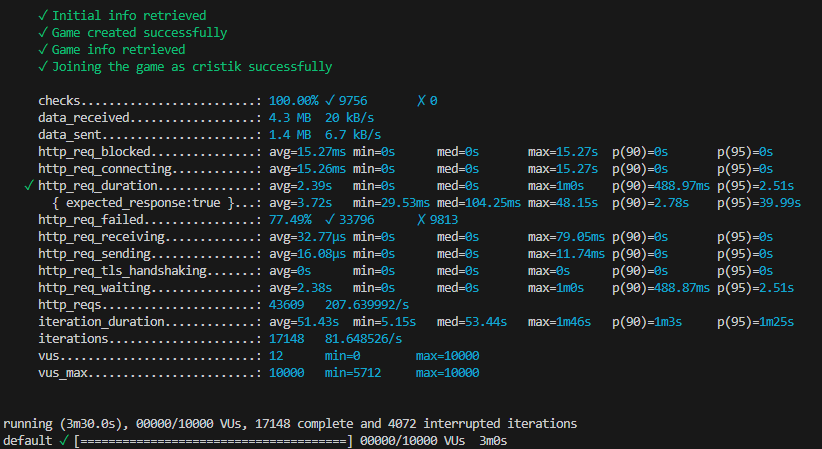
\includegraphics[width=1\textwidth]{Imatges/Tests/Núvol/4c-k6.png}  
    \caption{\textit{end-of-test summary} del Test 4 al núvol}
\end{figure}

\begin{figure}[!htbp]
    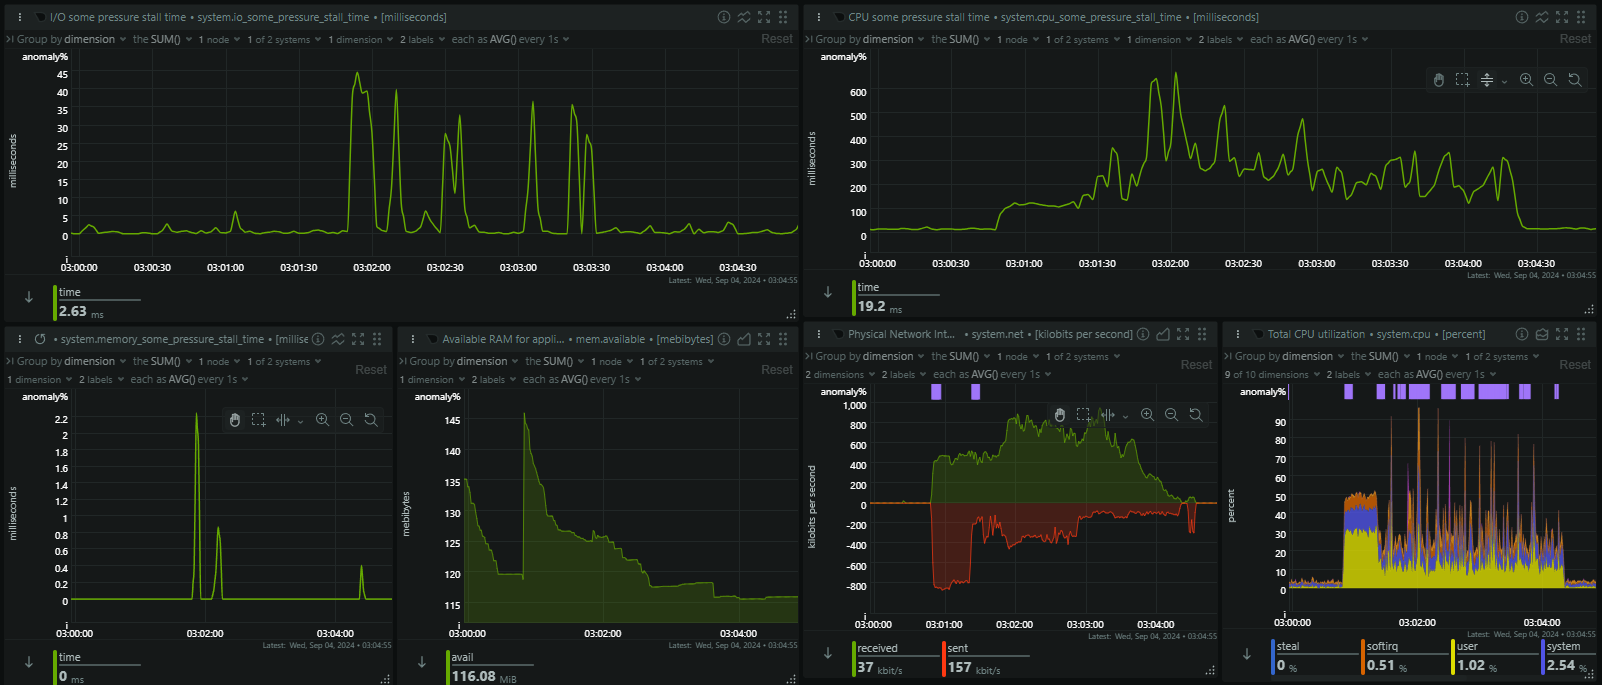
\includegraphics[width=1\textwidth]{Imatges/Tests/Núvol/4c-netdata.png}  
    \caption{Tauler de \textit{Netdata} del Test 4 al núvol}
\end{figure}

\subsubsection{Màquina local}
Consisteix en la següent comanda al \textit{Powershell}:
\begin{lstlisting}[language=bash, caption=Test 4 local]
    $env:K6_CLOUD=0; $env:K6_PRIMER=5000;$env:K6_MIG=10000; k6 run .\script.js
\end{lstlisting}

\begin{figure}[!htbp]
    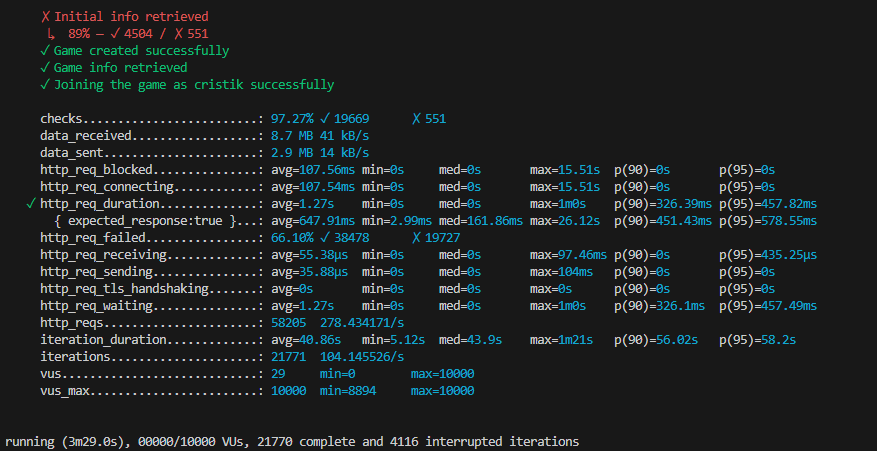
\includegraphics[width=1\textwidth]{Imatges/Tests/Local/4l-k6.png}  
    \caption{\textit{end-of-test summary} del Test 4 local}
\end{figure}

\begin{figure}[!htbp]
    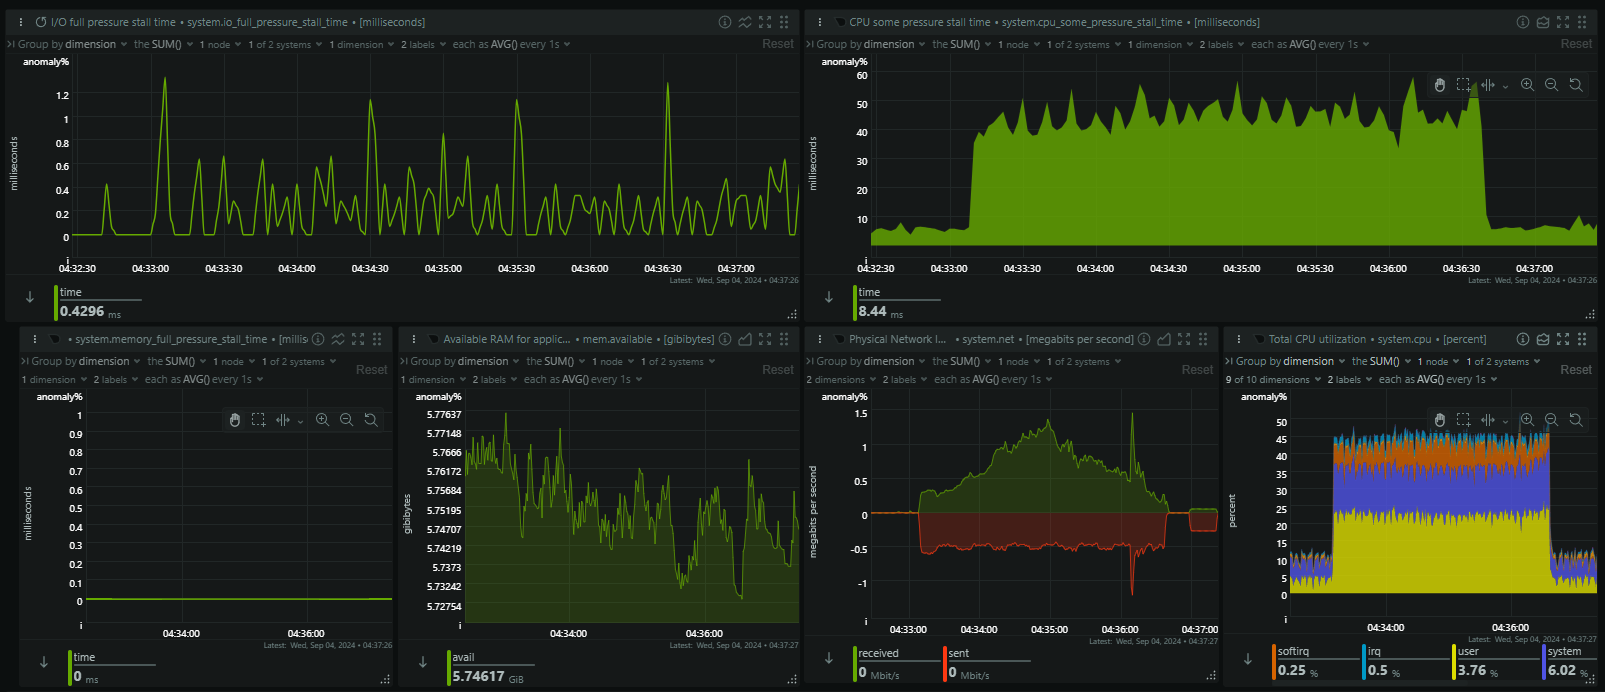
\includegraphics[width=1\textwidth]{Imatges/Tests/Local/4l-netdata.png}  
    \caption{Tauler de \textit{Netdata} del Test 4 local}
\end{figure}

\subsubsection{Conclusió del test}

En aquest test es pot observar una continuació de les observacions fetes en el Test 3. La màquina local continua sent aproximadament el doble de ràpida en mitjana en les peticions i, alhora, envia un percentatge menor de respostes amb més retràs que el \textit{threshold} o respostes fallides. Es manté la tendència que la màquina local processa més iteracions, amb un petit percentatge de \textit{checks} que fallen, mentre que la màquina al núvol continua realitzant menys \textit{checks}, però tots són correctes. Aquesta vegada, les dues màquines tenen un nombre similar d'iteracions interrompudes, cosa que podria suggerir que les peticions incorrectes a la màquina al núvol no arriben a ser processades a causa de ser descartades, resultant en més iteracions interrompudes.

Amb aquesta nova dada, es pot formular una altra hipòtesi: la diferència en la gestió dels \textit{checks} pot ser deguda a que la màquina local té una tolerància menor a la càrrega. En moments de saturació, podria optar per retornar un missatge d'error en lloc de processar les peticions, mentre que la màquina al núvol les guarda a la cua.

A \textit{Netdata}, es pot veure que la màquina local té una corba de connexió a Internet que s'ajusta a la càrrega en quant a dades rebudes, amb un pic aproximat de 1.3 Mbps. No obstant això, la quantitat de dades enviades es limita majoritàriament a 0.5 Mbps, cosa que no hauria de passar, ja que la quantitat de dades a enviar hauria de ser més alta que la de les dades rebudes. Donat que el retràs del processador es manté estable al voltant de 40 ms, una quantitat baixa, i la resta de les components generen un retràs negligible, es pot assumir que el rendiment de la màquina local està limitat per la connexió de pujada.

El mateix fenomen es pot observar a la màquina al núvol, tot i que aquí es nota un retràs significatiu al processador, que arriba fins a 650 ms. A més, hi ha alguns pics importants en l'entrada/sortida amb un retràs al voltant de 40 ms. Cal tenir en compte que el processador de la màquina al núvol es comparteix amb altres màquines virtuals, cosa que podria explicar per què es mostra una saturació i una capacitat al màxim, tot i que el gràfic pot indicar una utilització menor al 100\%. Això significa que el processador podria estar operant al límit de la seva capacitat, afectant el rendiment general de la màquina, encara que no es mostri com a completament saturat en les gràfiques de monitoratge.

\newpage
\subsection{Test 5}

El cinquè test té una càrrega gegant, que simula fins a 50000 usuaris generant una càrrega de treball cada 5 segons.

\subsubsection{Màquina al núvol}
Consisteix en la següent comanda al \textit{Powershell}:
\begin{lstlisting}[language=bash, caption=Test 5 al núvol]
    $env:K6_CLOUD=1; $env:K6_PRIMER=20000;$env:K6_MIG=50000; k6 run .\script.js
\end{lstlisting}

\begin{figure}[!htbp]
    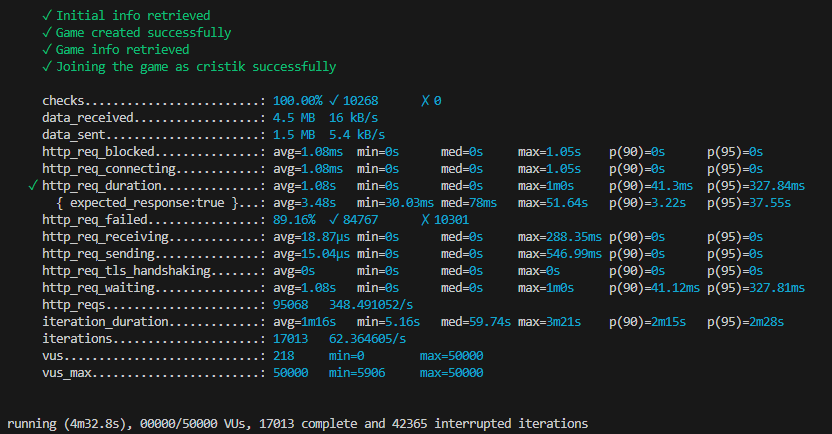
\includegraphics[width=1\textwidth]{Imatges/Tests/Núvol/5c-k6.png}  
    \caption{\textit{end-of-test summary} del Test 5 al núvol}
\end{figure}

\begin{figure}[!htbp]
    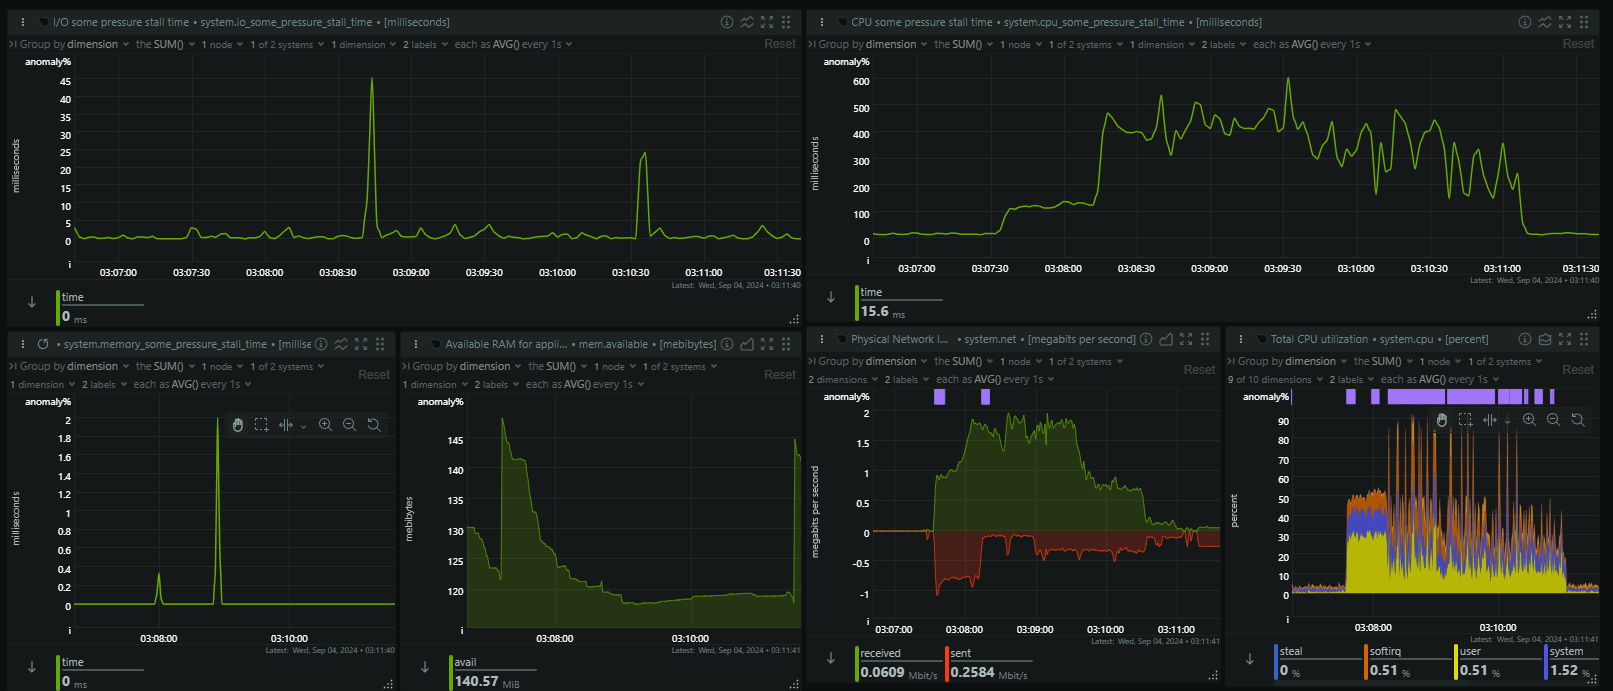
\includegraphics[width=1\textwidth]{Imatges/Tests/Núvol/5c-netdata.png}  
    \caption{Tauler de \textit{Netdata} del Test 5 al núvol}
\end{figure}

\subsubsection{Màquina local}
Consisteix en la següent comanda al \textit{Powershell}:
\begin{lstlisting}[language=bash, caption=Test 5 local]
    $env:K6_CLOUD=0; $env:K6_PRIMER=20000;$env:K6_MIG=50000; k6 run .\script.js
\end{lstlisting}

\begin{figure}[!htbp]
    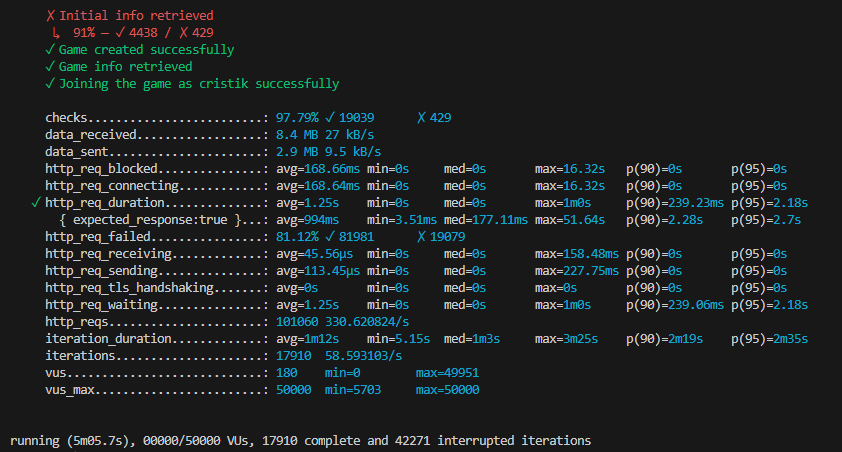
\includegraphics[width=1\textwidth]{Imatges/Tests/Local/5l-k6.png}  
    \caption{\textit{end-of-test summary} del Test 5 local}
\end{figure}

\begin{figure}[!htbp]
    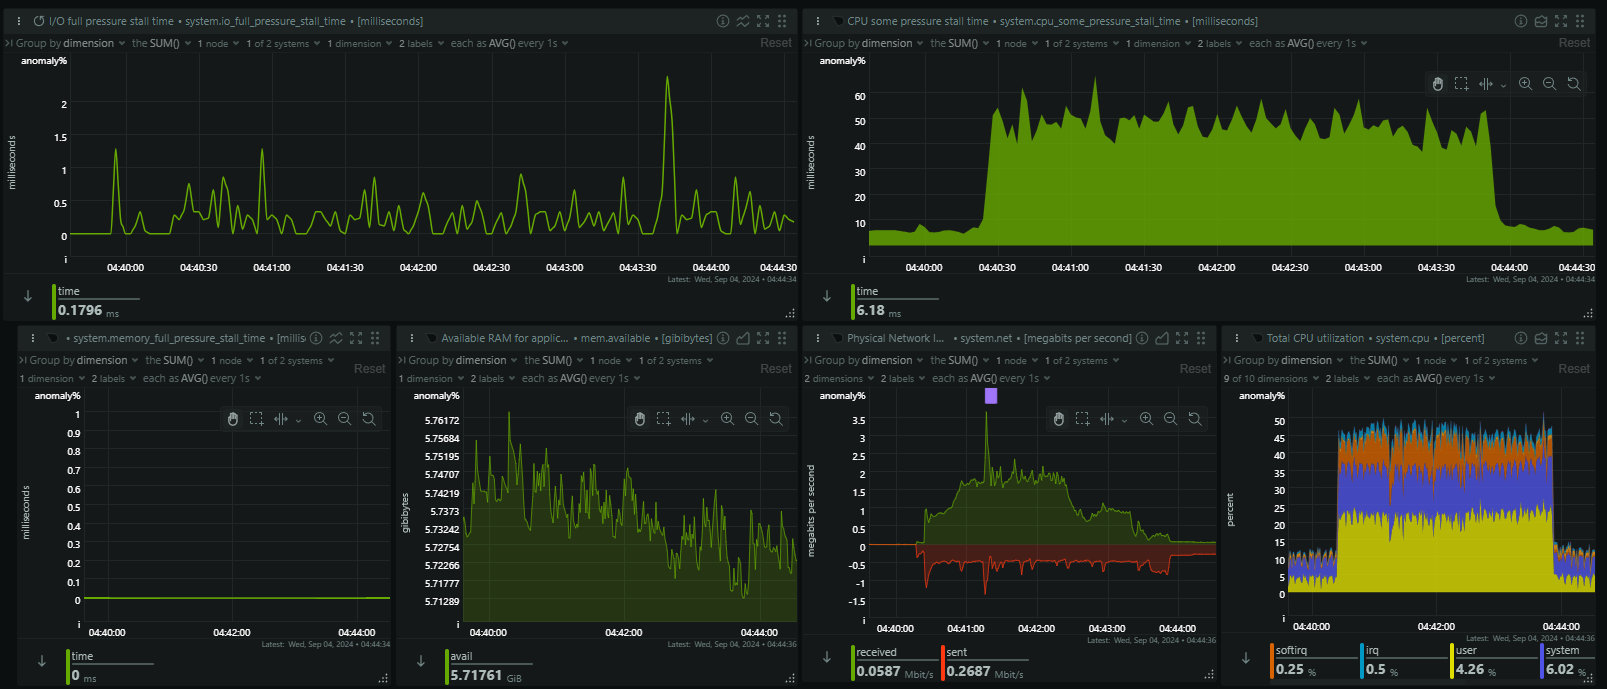
\includegraphics[width=1\textwidth]{Imatges/Tests/Local/5l-netdata.png}  
    \caption{Tauler de \textit{Netdata} del Test 5 local}
\end{figure}

\subsubsection{Conclusió del test}

En aquest test, es pot veure que s'ha arribat al punt en què els sistemes no són capaços de gestionar més \textit{VUs}, i per tant, la quantitat de peticions i \textit{checks} s'estanca. La quantitat de dades rebudes i enviades per segon decreix fins a un 20\% a la màquina al núvol en comparació amb el Test 4, tot i que el nombre de peticions correctes dins del \textit{threshold} es manté. D'altra banda, la quantitat de peticions fora del \textit{threshold} o incorrectes es dispara en els dos casos, pujant el percentatge d'aquestes respecte al Test 4 del 77,49\% a un 89,16\% a la màquina al núvol, i del 66,10\% a un 81,12\% a la màquina local.

D'altra banda, la mitjana de temps per rebre la resposta d'una petició s'ha mantingut respecte al Test 4 a la màquina local, mentre que a la màquina al núvol s'ha reduït de 2,39 segons a 1,08 segons. A partir d'aquest fet, es dedueix que el possible motiu pel qual, amb més càrrega, el temps de resposta disminueix és que les peticions que no han rebut resposta no es comptabilitzen, i en augmentar massivament la càrrega, es polaritza el temps de resposta: la gran majoria de peticions o bé reben una resposta relativament ràpida, o no en reben cap. Aquest fet es pot comprovar mirant la mediana i els percentils. Efectivament, la mediana de resposta és de 0 segons (no ha rebut cap resposta). Alhora, a la màquina al núvol, on abans, al Test 4, el 95\% de els \textit{VUs} acabaven de mitjana les peticions en menys de 2,51 segons, al Test 5 ho fan en menys de 0,427 segons, mostrant un altre cop la polarització: les peticions que arriben a ser contestades ho fan en poc temps, però la gran majoria de la resta no arriben a ser-ho.

Pel que fa al rendiment de les diferents peces de les màquines, s'observa al \textit{Netdata} que la màquina local presenta característiques gairebé idèntiques a les del Test 4, amb una latència baixa de 60 ms per part del processador i una latència negligible per part de la resta de components. Això reforça la idea que el coll d'ampolla en aquesta màquina és la velocitat de pujada. Pel que fa a la màquina al núvol, s'observa el mateix fenomen que en el Test 4: una elevada latència provocada pel retard del processador, la qual cosa limita l'enviament de dades a través de la seva connexió a internet.

Per assegurar-se que l'amplada de banda no és el factor limitant de la màquina client, s'ha instal·lat i executat el test de velocitat \textit{Speedtest CLI} amb les següents comandes: 
\begin{lstlisting} 
curl -s https://packagecloud.io/install/repositories/ookla/speedtest-cli/script.deb.sh | sudo bash 
sudo apt-get install speedtest 
speedtest 
\end{lstlisting} 
La resposta ha estat la següent:

\begin{figure}[!htbp] 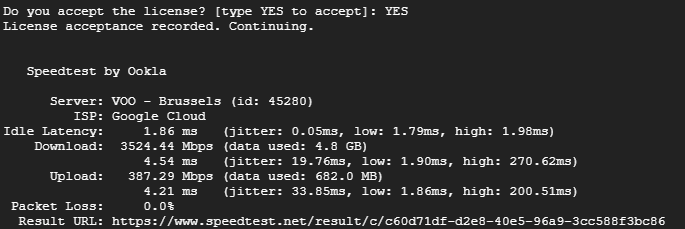
\includegraphics[width=1\textwidth]{Imatges/speedTest.png}
\caption{Test de velocitat de la màquina al núvol} \end{figure}

Amb això es pot confirmar que l'amplada de banda disponible és molt superior a la que ha utilitzat la màquina al núvol durant aquest Test 5. Per tant, el factor limitant és probablement el processador

A més a més, minuts després d'acabar el test, han arribat tres correus de l'aplicació \textit{Netdata}, en la qual s'havia creat un compte mentre s'exploraven les seves possibilitats.

\begin{figure}[!htbp] 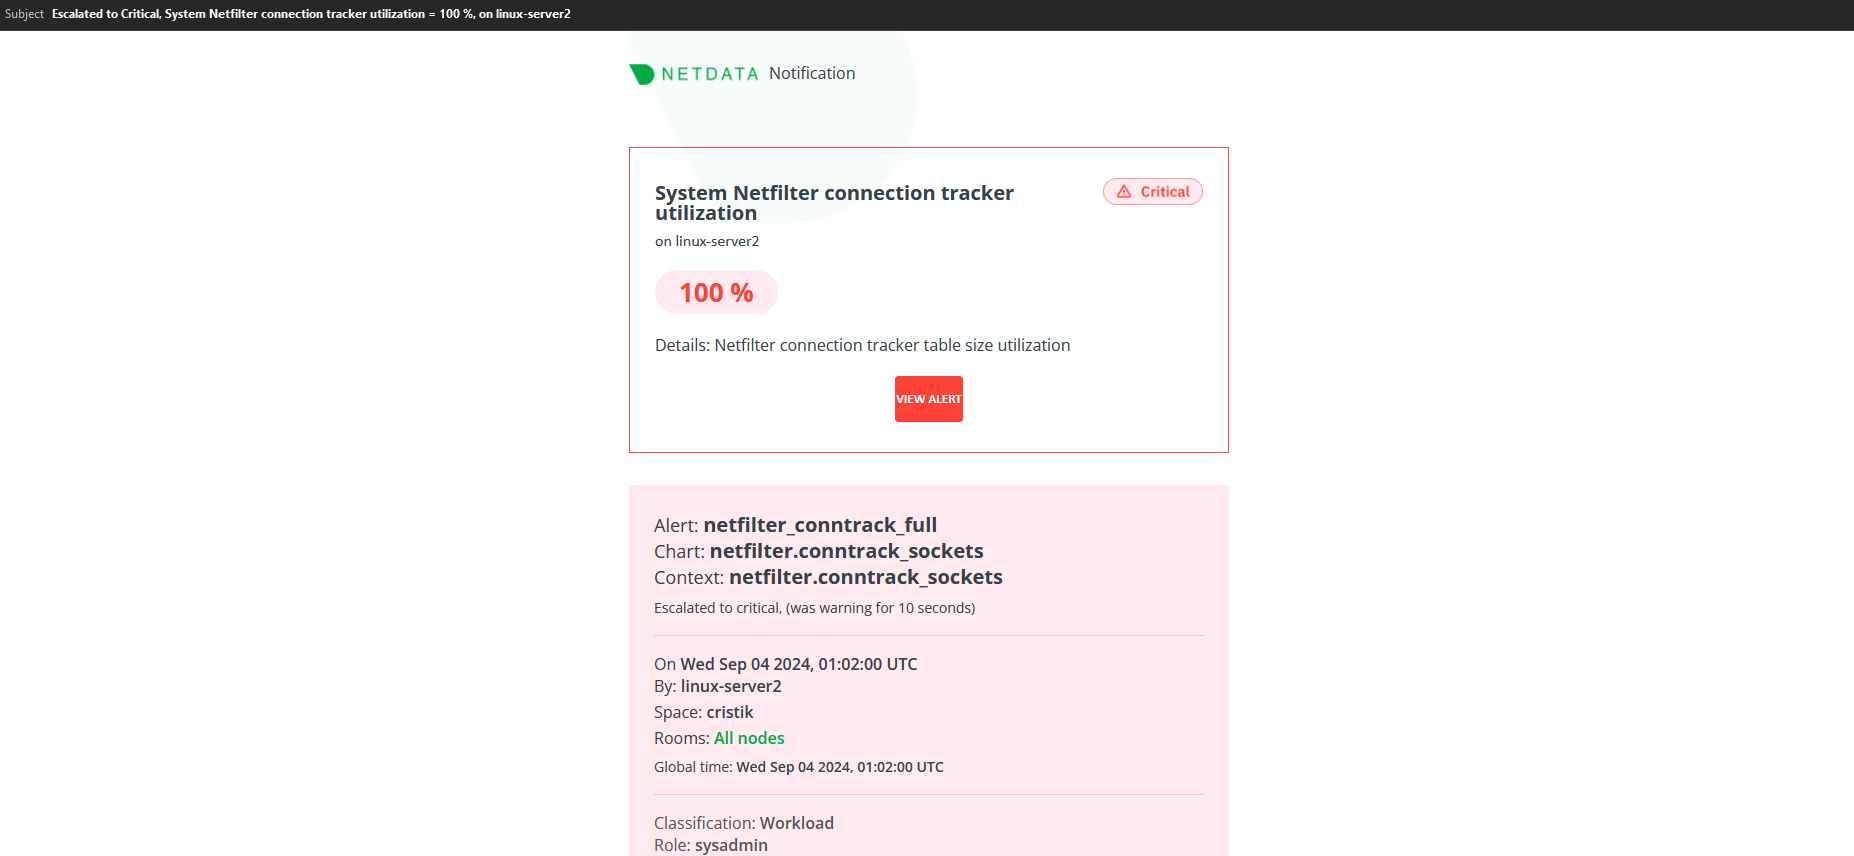
\includegraphics[width=1\textwidth]{Imatges/mail-netdata.png}
\caption{Alerta de \textit{Netdata} al correu electrònic} \end{figure}

En prémer el botó per veure l'alerta, s'ha pogut observar amb més detall quin era el problema a la pàgina web de \textit{Netdata}. El Test 5 havia esgotat el límit de connexions possibles que permetia la màquina, que en aquest cas era d'aproximadament 7.689 connexions. Amb aquesta informació, podem estar segurs que la màquina al núvol no ha estat capaç de connectar amb tots els \textit{VUs}.

\begin{figure}[!htbp] 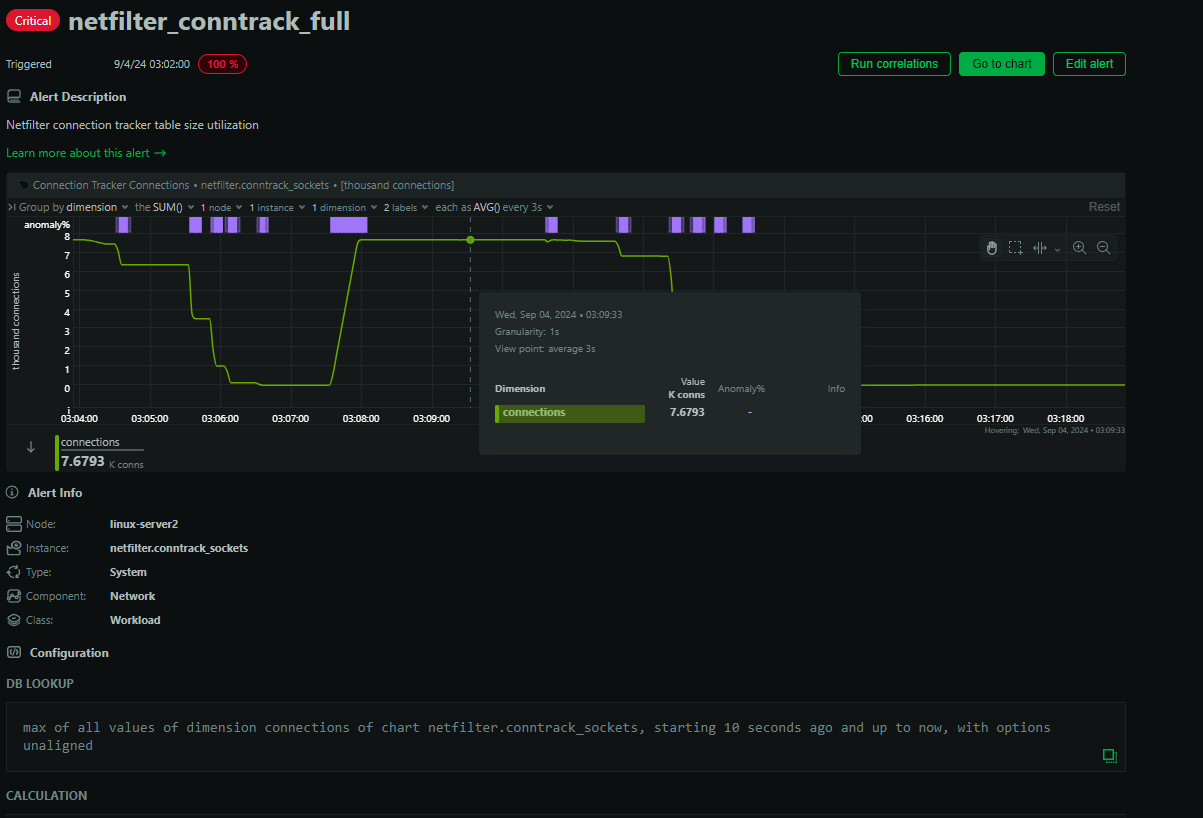
\includegraphics[width=1\textwidth]{Imatges/Tests/Núvol/5c-alerta.png}
\caption{Alerta de \textit{Netdata} durant el Test 5 al núvol} \end{figure}